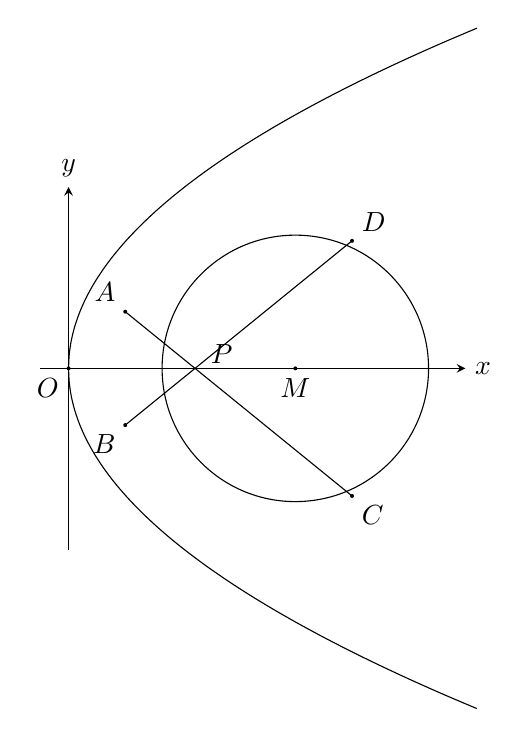
\begin{tikzpicture}[scale=.72,>=stealth]
\draw[->] (-.5,0)--(7,0) node[right] {$x$};
\draw[->] (0,-3.2)--(0,3.2) node[above] {$y$};
\draw[domain=0:6,smooth,variable=\x] plot ({\x*\x/5},{\x});
\draw[domain=0:6,smooth,variable=\x] plot ({\x*\x/5},{-\x});
\draw (4,0) circle (2.35);
\coordinate (A) at (1.0,1.0); \coordinate (B) at (1.0,-1.0);
\coordinate (C) at (5.0,-2.25); \coordinate (D) at (5.0,2.25);
\draw (A)--(C) (B)--(D);
\fill (0,0) circle (1pt) node[below left] {$O$};
\fill (4,0) circle (1pt) node[below] {$M$};
\fill (A) circle (1pt) node[above left] {$A$};
\fill (B) circle (1pt) node[below left] {$B$};
\fill (C) circle (1pt) node[below right] {$C$};
\fill (D) circle (1pt) node[above right] {$D$};
\node at (2.7,.25) {$P$};
\end{tikzpicture}
